\documentclass[12pt]{article}

\usepackage{graphicx}
\usepackage{caption}
\usepackage{float}
\usepackage{subcaption}

\usepackage{amsmath}
\usepackage{algorithm}
\usepackage[noend]{algpseudocode}

\makeatletter
\def\BState{\State\hskip-\ALG@thistlm}
\makeatother

\usepackage{hyperref}



\usepackage{xepersian}

\settextfont{XB Zar}[
  Path=./fonts/,
  Scale=1.2,
  Extension=.TTF,
  UprightFont=*,
  ItalicFont=*It,
  BoldFont=*Bd,
  BoldItalicFont=*BdIt
]

\setlatintextfont[Scale=1.1]{Times New Roman}

\setmonofont[
  Path=./fonts/,
  Scale=1.0,
  Weight=800,
  Extension=.TTF,
]{Inconsolata}

\title{مقایسه الگوریتم‌های مرتب‌سازی}
\author{محمد ترابی - علی جعفر‌آبادی - رضا تاج‌گذاری} 
\date{\today}

\begin{document}
\maketitle

\section{مرتب‌سازی انتخابی}

سلام این یک متن تستی است


\begin{algorithm}
  \caption{مرتب‌سازی انتخابی}\label{euclid}
  \begin{latin}
    \begin{algorithmic}[1]
      \Procedure{MyProcedure}{}
      \State $\textit{stringlen} \gets \text{length of }\textit{string}$
      \State $i \gets \textit{patlen}$
      \BState \emph{top}:
      \If {$i > \textit{stringlen}$} \Return false
      \EndIf
      \State $j \gets \textit{patlen}$
      \BState \emph{loop}:
      \If {$\textit{string}(i) = \textit{path}(j)$}
      \State $j \gets j-1$.
      \State $i \gets i-1$.
      \State \textbf{goto} \emph{loop}.
      \State \textbf{close};
      \EndIf
      \State $i \gets i+\max(\textit{delta}_1(\textit{string}(i)),\textit{delta}_2(j))$.
      \State \textbf{goto} \emph{top}.
      \EndProcedure
    \end{algorithmic}
  \end{latin}
\end{algorithm}

\section{مرتب‌سازی درجی}

اگر یک دسته کارت به شما داده شود که اعداد ۱ تا ۵۰ روی آن نوشته شده است، چگونه آن را مرتب می‌کنید؟
احتمالا اول تعداد کمی کارت برمی‌دارید و آن را مرتب می‌کنید؛
سپس بقیه کارت‌ها را یکی پس از دیگری نگاه می‌کنید
و در جای مناسب میان کارت‌های مرتب شده قرار می‌دهید.
شکل ۱ نمایی کلی از این روش مرتب‌سازی نشان می‌دهد.

وقتی کارت‌ها را با این روند مرتب می‌کنیم، همواره تعدادی از کارت‌ها مرتب شده است و کارت‌هایی که هنوز مرتب نشده، یکی پس از دیگری
در دستهٔ کارت‌های مرتب شده درج می‌شوند.
اگر با این روش کارت‌ها را مرتب کنیم، درواقع از مرتب‌سازی درجی استفاده کرده ایم.

\begin{figure}[!h]
  \centering
  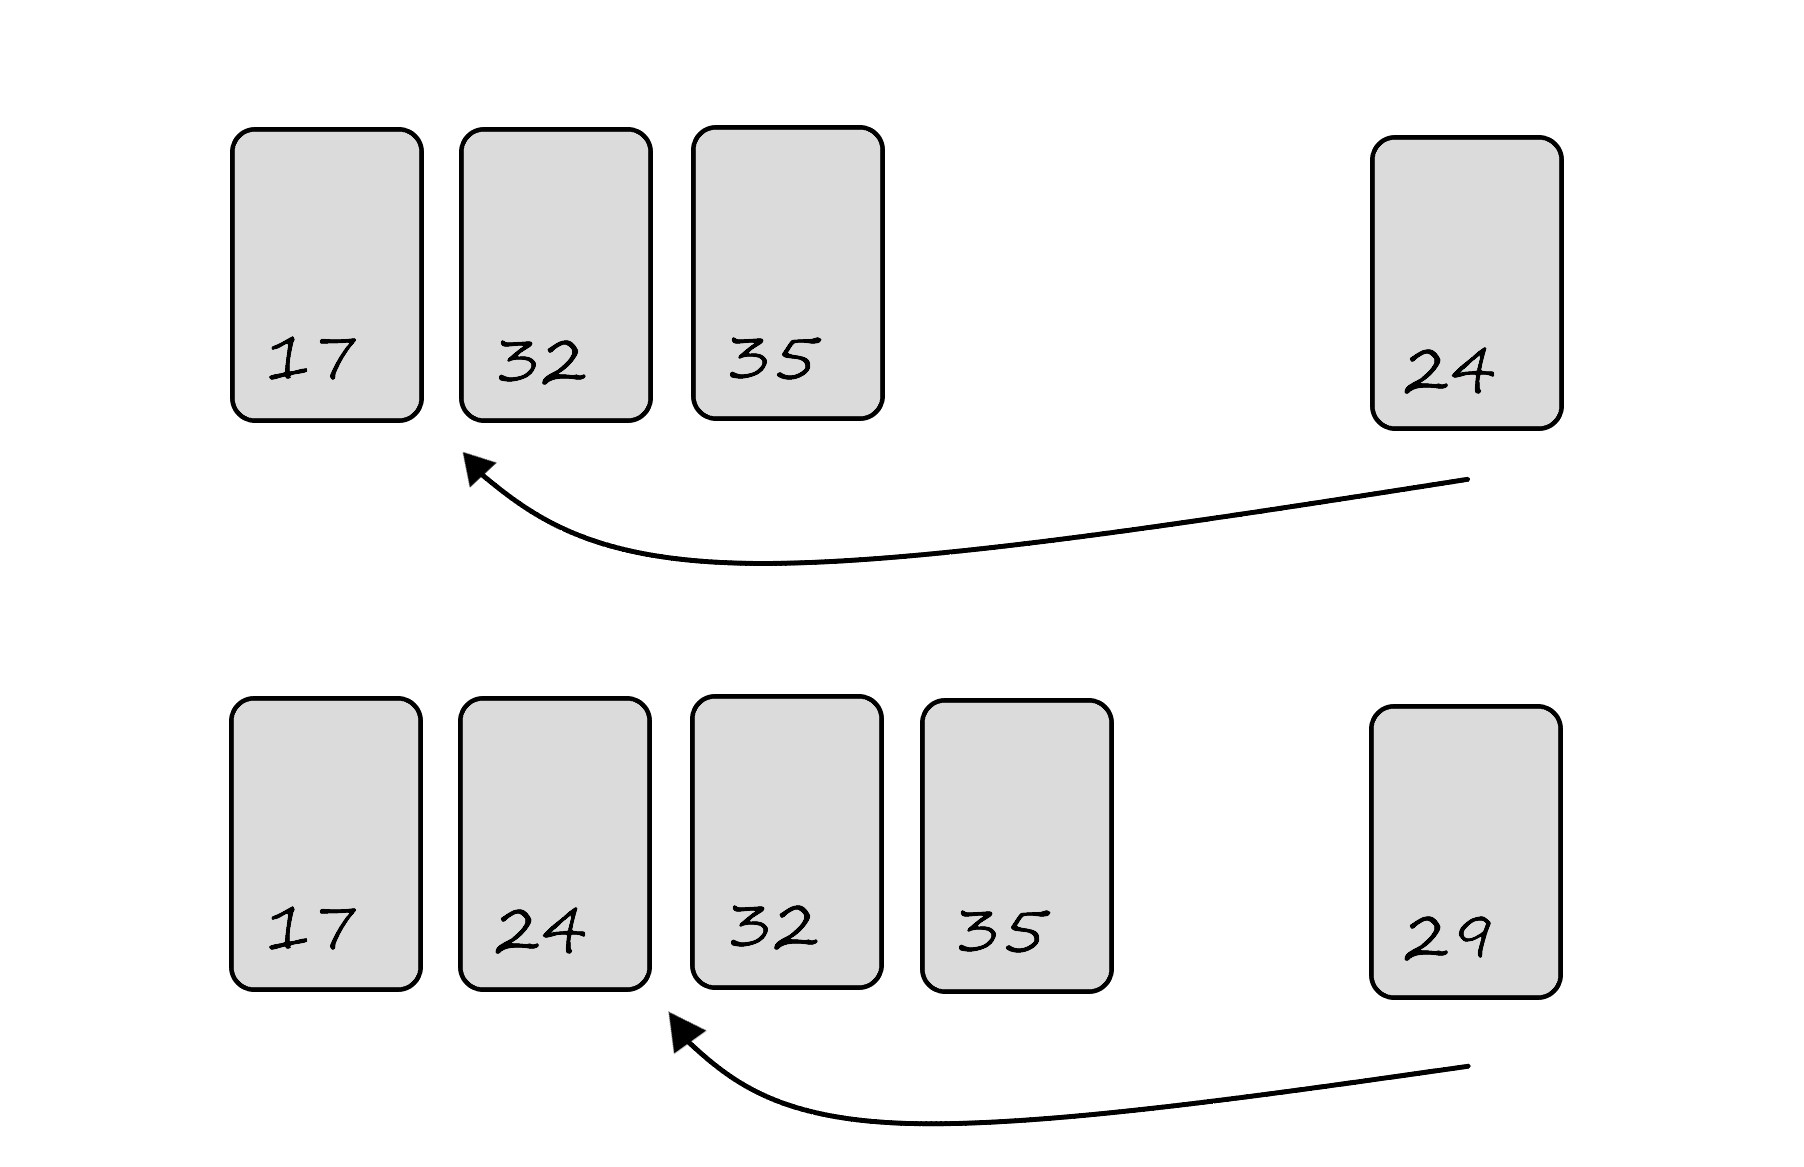
\includegraphics[width=.8\textwidth]{figs/sortingCards2.jpg}
  \caption{
    مرتب کردن کارت‌ها به کمک مرتب‌سازی درجی
  }
  \label{fig:app1}
\end{figure}

\begin{algorithm}
  \caption{مرتب‌سازی درجی}\label{euclid}
  \begin{latin}0
    \begin{algorithmic}[1]
      \Procedure{MyProcedure}{}
      \State $\textit{stringlen} \gets \text{length of }\textit{string}$
      \State $i \gets \textit{patlen}$
      \BState \emph{top}:
      \If {$i > \textit{stringlen}$} \Return false
      \EndIf
      \State $j \gets \textit{patlen}$
      \BState \emph{loop}:
      \If {$\textit{string}(i) = \textit{path}(j)$}
      \State $j \gets j-1$.
      \State $i \gets i-1$.
      \State \textbf{goto} \emph{loop}.
      \State \textbf{close};
      \EndIf
      \State $i \gets i+\max(\textit{delta}_1(\textit{string}(i)),\textit{delta}_2(j))$.
      \State \textbf{goto} \emph{top}.
      \EndProcedure
    \end{algorithmic}
  \end{latin}
\end{algorithm}


\end{document}